\section{Modèle de comportement du solide}
\begin{obj}
Il s'agit de déterminer une équation différentielle permettant de de modéliser le comportement du fuselage 1.
\end{obj}

\subsubsection*{Notations et hypothèses}
\begin{itemize}
\item Les notations sont fournies sur la figure \ref{fig_sia2014_02}. 
\item Le repère Rg : $\repere{O}{x_g}{y_g}{z_g}$ est un repère galiléen. 
\item Le problème est plan dans le plan de symétrie géométrique $\left(O,\vect{z_g},\vect{x_g}\right)$. En conséquence les solides 4 et 5
représentent deux vérins amortisseurs avec des caractéristiques $k$ et $\lambda$ doubles des caractéristiques d'un seul 
vérin amortisseur. 

\item L'hypothèse faite sur l'angle $\beta$ conduit à considérer que $\vect{CD}$ est constamment colinéaire à $\vect{z_g}$, soit 
$\vect{CD} = \ell \vect{z_g}$. 

\item Le mouvement du solide 1 est réduit à un mouvement de translation vertical. En conséquence la roue 6 est 
fixe dans le repère galiléen. 

\item On rappelle que la masse des solides 3, 4, 5, 6 est négligée devant la masse des solides 1 et 2. 

\item On suppose toutes les liaisons énergétiquement parfaites. 

\item La liaison pivot entre 1 et 2 aussi bien que la liaison pivot glissant entre 4 et 5 sont actionnées par des ressorts 
de raideurs respectives $k_{\theta}$ et $k$ et amorties en parallèle aux ressorts avec des facteurs d'amortissement $\lambda_{\theta}$ et $\lambda$. 

Dans ces conditions, pour la liaison pivot entre 1 et 2, on note le couple de rappel élastique $\vect{C_r}(1\rightarrow 2) = C_r \vect{y_g}$ avec $C_r =-k_{\theta} \theta$, et le couple d'amortissement $\vect{C_v}(1\rightarrow 2) = C_v \vect{y_g}$ avec $C_v= -\lambda_{\theta} \thetap$

De même pour la liaison pivot glissant entre 4 et 5, on note la force de rappel élastique $\vect{F_r}(4\rightarrow 5) = F_r \vect{z_g}$ avec 
$F_r = -k \left( \ell - \ell_0\right)$ où $\ell_0$ est la valeur de $\ell$ quand le ressort est à vide, et la force d'amortissement $\vect{F_v}(4\rightarrow 5) = F_V \vect{z_g}$ avec $F_v = -\lambda\dot{\ell}$.

\end{itemize}

\question{Déterminer l'équation du mouvement du système.}


\section{Structure de la commande asservie de l'amortisseur semi-actif}
\begin{obj}
Valider le choix du constructeur de contrôler les accélérations du pylône de queue mpar la maîtrise du mouvement de la cabine.
\end{obj}

L'équation de comportement de la cabine est donnée par l'équation suivante : 
$$
m_2 L^2 \ddot{\theta}^{\star} + \lambda_{\theta} \thetap^{\star} + k_{\theta}\theta^{\star} = m_2 L \ddot{z}.
$$

On rappelle si nécessaire que dans cette relation, $\theta^{\star} = \theta - \theta_0$ représente la variation angulaire de la queue par rapport à sa position à l’équilibre $\theta_0$. $\thetap^{\star}$ et $\thetapp^{\star}$
sont ses dérivées successives par rapport au temps, et $\ddot{z}$ est l’accélération absolue de la cabine (voir figure \ref{fig_sia2014_03}).

\question{Montrer qu’à décélération constante de la cabine, l’accélération de la queue tend vers zéro en régime établi.}

\question{En admettant que l’accélération de la queue est maximale à l’instant initial, déterminer son expression notée $\thetapp_{\text{max}}$ en fonction de $A_0$, et $L$. Conclure sur le choix du constructeur de contrôler la décélération de la cabine.}


\question{On donne la réponse indicielle du système. Proposer un modèle de comportement du système.}

\begin{center}
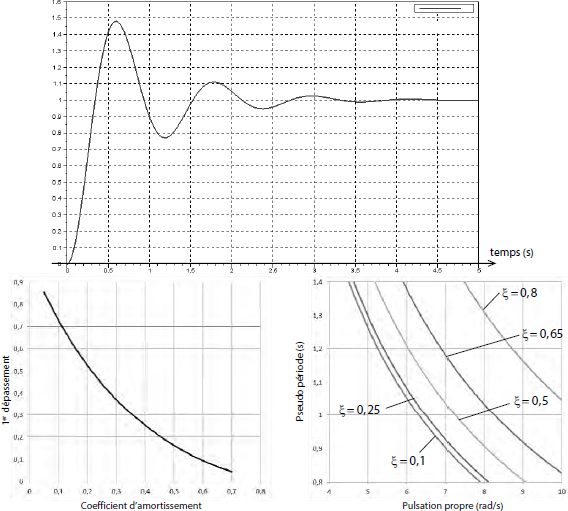
\includegraphics[width=\linewidth]{dr}
\end{center}